\section{从增长、衰减与振动说起}
\label{sec:15-Differential-Equations-and-Dynamical-Systems/01-ODE-Theory/01}

一间药品冷库的温控手册上写着这样一行：制冷停机后，库温每分钟上升的速度正比于库内外温差。值班表要问的却是另一件事：凌晨两点断电，到抢修队五点赶到，药品会不会越过 \(8\,^{\circ}\mathrm{C}\) 的红线。手册给的是每一瞬间的变化率，排班要的是三个小时后的那一个数。中间隔着一整条轨迹。

这个落差是本 Part 的起点。微分方程写下的永远是局部规则——此刻的状态决定此刻的变化方向；而使用者要的是这条规则递推到底之后的整体形状。把微分方程当成``一类需要凑技巧的函数题''，就会漏掉这层由局部到整体的关系。

\subsection{建模先给出变化率，很少直接给出轨迹}

想一想那些最早被写成方程的现象。资源充裕时人口的增长率近似正比于当前规模；放射性物质单位时间衰变的比例是常数；电容器放电的电流正比于剩余电荷。三句话说的都是变化率 \(x'(t)\) 与当前状态 \(x(t)\) 的关系，谁也没有说出 \(x(t)\) 的形状。精确化之后，它们是同一个方程

\[
x'(t)=k\,x(t).
\]

解是

\[
x(t)=x_0e^{kt},
\qquad x_0=x(0).
\]

有两件事值得停一下。单凭方程 \(x'=kx\) 得到的是一族曲线，每个初值 \(x_0\) 给出一条；初值条件负责从这族曲线里挑出唯一的一条。``初值问题''这个词说的正是这两步的合取：方程管形状，初值管落点。

\(k>0\) 时解指数增长，\(k<0\) 时指数衰减。两条不同的解曲线永不相交——从 \(x_0=1\) 出发的解永远是从 \(x_0=2\) 出发的解的一半。这个观察很朴素，却预告了本单元第三节的核心问题：解曲线总能把平面这样整齐地梳理开吗？

冷库温度里藏着同一个结构。把整间库房近似成温度均匀的单一状态 \(T(t)\)，热平衡给出

\[
C\frac{dT}{dt}
=k\bigl(T_{\mathrm{out}}-T\bigr)
-\eta u+w,
\]

其中 \(C\) 是有效热容量，\(T_{\mathrm{out}}\) 是外温，\(u\) 是制冷输入，\(w\) 汇总开门、货物进出等热扰动。先把外温、输入和扰动视为常数，平衡温度为

\[
T_{\mathrm{eq}}
=T_{\mathrm{out}}-\frac{\eta}{k}u+\frac{w}{k},
\]

令偏差 \(e=T-T_{\mathrm{eq}}\)，方程立刻塌缩成

\[
e'=-\frac{k}{C}e.
\]

于是库温以时间常数 \(C/k\) 指数地回到平衡；断电意味着 \(u=0\)，新的 \(T_{\mathrm{eq}}\) 抬到接近外温，剩下的只是算一个指数何时越线。这里值得保留的不止解公式。把冷库压缩成单一温度、把 \(C\) 与 \(k\) 当常数，已经决定了模型看不见门边与货架深处的空间温差。方程会把选定的机制推演到底，却不会替建模者判断被省略的那部分是否致命。

\subsection{增长撞上资源上限时，指数律必须让位}

指数增长有一个显然的失效情形：任何真实环境都装不下无限多的个体。增长率``正比于当前规模''只在资源充裕时成立，种群接近环境能支撑的极限时，增长必须慢下来。

把``相对增长率随规模线性下降''这一最省事的修正代进去，得到 Logistic 方程

\[
x'=rx\Bigl(1-\frac{x}{K}\Bigr),
\]

其中 \(r>0\) 是低密度下的固有增长率，\(K>0\) 称为承载力。两个极端一望可知：\(x\) 远小于 \(K\) 时括号接近 \(1\)，方程退回 \(x'=rx\)；\(x\) 接近 \(K\) 时括号接近 \(0\)，增长趋于停止。

分离变量可解。由

\[
\frac{dx}{x(1-x/K)}=r\,dt
\]

出发，左边拆成部分分式后积分，

\[
\begin{aligned}
\frac{1}{x(1-x/K)}
&=\frac1x+\frac{1/K}{1-x/K},\\
\ln\frac{x}{1-x/K}
&=rt+C,\\
x(t)
&=\frac{K}{1+Ae^{-rt}},
\qquad
A=\frac{K-x_0}{x_0}.
\end{aligned}
\]

公式值得逐条读。无论 \(x_0\) 多小（只要为正），\(t\to\infty\) 时都有 \(x(t)\to K\)：承载力是方程自己推出来的长期归宿，不必作为外部上限硬加进去。若 \(x_0>K\)，例如一次过量迁入，则 \(A<0\)，解从上方衰减回 \(K\)。\(x_0=0\) 时 \(A\) 无定义——直接代回方程可见 \(x\equiv0\) 与 \(x\equiv K\) 都是常数解，称为平衡解：种群灭绝则永远灭绝，恰好满员则永远满员。

两个平衡的地位并不对等。\(K\) 附近的扰动会被拉回去，\(0\) 附近的扰动会被放大。同为平衡，一个吸引、一个排斥，这个差异到下一单元会长成整套稳定性理论。

\subsection{方向场让你不解方程就看见解}

换一副眼睛。方程 \(x'=f(t,x)\) 的右端在平面上每个点 \((t,x)\) 处给出一个确定的斜率。在一批点上画出以该斜率为方向的小线段，就得到方向场。解曲线经过任何一点时都必须与该点的线段相切，于是顺着线段走，就能徒手描出解的形状。

\begin{center}
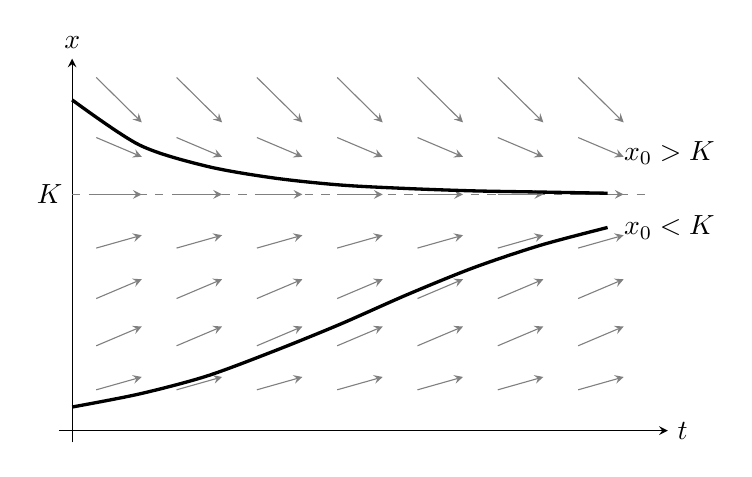
\begin{tikzpicture}[>=stealth,xscale=1.7,yscale=1.5]
  \draw[->] (-0.1,0) -- (4.45,0) node[right] {\(t\)};
  \draw[->] (0,-0.1) -- (0,3.15) node[above] {\(x\)};
  \draw[dashed,gray] (0,2) -- (4.3,2);
  \node[left] at (0,2) {\(K\)};
  \foreach \tt in {0.35,0.95,1.55,2.15,2.75,3.35,3.95}{
    \foreach \xx/\ss in {0.4/0.32,0.8/0.48,1.2/0.48,1.6/0.32,2.0/0,2.4/-0.48,2.8/-1.12}{
      \draw[thin,gray,->] ({\tt-0.17},{\xx-0.17*\ss}) -- ({\tt+0.17},{\xx+0.17*\ss});
    }
  }
  \draw[very thick] plot[smooth] coordinates
    {(0,0.20) (0.5,0.31) (1,0.46) (1.5,0.67) (2,0.90) (2.5,1.15) (3,1.38) (3.5,1.57) (4,1.72)};
  \draw[very thick] plot[smooth] coordinates
    {(0,2.80) (0.5,2.42) (1,2.24) (1.5,2.14) (2,2.08) (2.5,2.05) (3,2.03) (3.5,2.02) (4,2.01)};
  \node[right] at (4.05,1.72) {\(x_0<K\)};
  \node[right] at (4.05,2.35) {\(x_0>K\)};
\end{tikzpicture}
\end{center}

\emph{Logistic 方程的方向场：两条粗线是解，它们只是顺着灰色小箭头走出来的。}

图上没有出现任何解公式。\(x=0\) 与 \(x=K\) 两条水平线上斜率为零，\(0<x<K\) 区域斜率为正且在 \(x=K/2\) 附近最陡，\(x>K\) 区域斜率为负——单看这些小箭头，前面花了一页积分才得到的定性结论已经全在眼前：正初值的解一律上升并弯向 \(K\)，超出 \(K\) 的解回落到 \(K\)，两条平衡线一推一拉。

方向场还把存在唯一性问题几何化了。若每点的方向都组织良好，解曲线就像水流一样铺满平面且互不相交；唯一性失效在图上的样子是某点处分叉出多条流线，水流在那里不知道该往哪边去。本单元第三节的两个反例，都可以先在这样一张图上用眼睛看穿。

\subsection{振动需要两个状态变量}

弹簧振子（或单摆的小角度近似）满足

\[
x''+\omega^2x=0,
\]

加速度正比于位移且指向平衡点。这是二阶方程：变化率的变化率与状态相关。

标准手法是先降阶。令 \(v=x'\)，把速度也算作状态的一部分，则

\[
x'=v,
\qquad
v'=-\omega^2x.
\]

为什么必须补上 \(v\)？单看 \(x\) 无法预测未来，同一个位置可以以不同速度经过，方向场在 \((t,x)\) 平面上根本画不出来——一个点对应不止一个斜率。补上 \(v\) 之后，``现在''才完整地决定``下一步''，前一小节那张图才重新可画，只不过要画在 \((x,v)\) 平面上。动力系统的状态几乎总是包含速度类变量，原因就在这里。

方程组的解是

\[
x(t)=x_0\cos\omega t+\frac{v_0}{\omega}\sin\omega t,
\qquad
v(t)=x'(t).
\]

在 \((x,v)\) 平面上，轨迹是绕原点的闭合椭圆，位置与速度此消彼长、周期性互换。这个以状态为坐标轴、把时间退到幕后的平面，是下一单元\hyperref[sec:15-Differential-Equations-and-Dynamical-Systems/02-Stability-and-Dynamical-Systems/01]{``相平面：把解画成几何''}的主角。

把方程组写成矩阵形式

\[
\begin{pmatrix}x'\\v'\end{pmatrix}
=
\begin{pmatrix}0&1\\-\omega^2&0\end{pmatrix}
\begin{pmatrix}x\\v\end{pmatrix},
\]

它是线性系统 \(u'=Au\) 的第一个非平凡例子。下一节要回答的问题已经摆在那里：这类系统的解能不能像 \(x'=kx\) 那样，写成某种指数。

\subsection{能写出公式的方程是少数}

至此的三个模型都有显式解，这是精心挑选的结果。多数微分方程没有初等函数形式的解。右端只是普通函数的 \(x'=e^{-t^2}\)，其解也只能写成积分（误差函数就是这样定义出来的）；\(x'=\sin(tx)\) 没有已知的封闭解；绝大多数非线性方程更是如此。

承认这一点，理论的任务就分成两支。一支把能彻底解出的那一类——线性系统——研究到底，做成后续一切分析的样板，这是下一节的事。另一支面对解不出公式的方程，发展不依赖公式仍能断言性质的推理：解是否存在、是否唯一（本单元第三节），长期行为是什么形状（下一单元）。方向场那张图已经示范了后一支的做法：定性理论是主要工具，不是解析求解失败之后的退路。
